\documentclass{beamer}
% Required packages
\usepackage{amsmath}
\usepackage{physics}
\usepackage{graphicx}
\usepackage{siunitx}
\usepackage{xcolor}
% Set image search paths
\graphicspath{{../images/}{../../shared/images/}}

% Define custom colors for DS9 theme
\definecolor{ds9blue}{RGB}{25,25,112}
\definecolor{ds9gold}{RGB}{218,165,32}
\definecolor{ds9grey}{RGB}{105,105,105}
\definecolor{ds9red}{RGB}{178,34,34}
% Set up the Madrid theme with custom colors
\usetheme{Madrid}
\usecolortheme{whale}
\setbeamercolor{palette primary}{bg=ds9blue,fg=white}
\setbeamercolor{palette secondary}{bg=ds9grey,fg=white}
\setbeamercolor{palette tertiary}{bg=ds9gold,fg=black}
\setbeamercolor{palette quaternary}{bg=ds9red,fg=white}
\setbeamercolor{structure}{fg=ds9blue}
\setbeamercolor{title}{fg=ds9gold}
\setbeamercolor{subtitle}{fg=ds9gold}
\setbeamercolor{frametitle}{bg=ds9blue,fg=white}
\setbeamercolor{block title}{bg=ds9blue,fg=white}
\setbeamercolor{block body}{bg=ds9grey!20,fg=black}

\title[NOPS Guide]{NOPS Answer Sheet Guide}
\subtitle{Professional Exam Completion Standards}
\author[Mr. Gullo]{Mr. Gullo}
\date[June 2025]{June, 2025}

\begin{document}

\frame{\titlepage}

\begin{frame}{Learning Objectives}
\frametitle{Learning Objectives}
By the end of this guide, you will be able to:
\begin{itemize}
\item Properly handle and maintain your NOPS answer sheet
\item Complete personal information and registration accurately
\item Apply correct marking techniques for optimal scanning
\item Follow appropriate error correction protocols
\end{itemize}
\end{frame}

\begin{frame}{Essential Requirements}
\frametitle{NOPS System Requirements}
\begin{block}{Critical Materials}
\begin{itemize}
\item \textbf{Blue or black pen only} (no pencils or erasers)
\item Clean, flat working surface
\item Careful attention to detail
\end{itemize}
\end{block}

\begin{block}{Answer Sheet Care}
\begin{itemize}
\item Keep sheet clean, dry, and flat at all times
\item Avoid folding, creasing, or damaging the paper
\item Handle with clean hands only
\end{itemize}
\end{block}
\end{frame}

\begin{frame}{Registration Number Process}
\frametitle{Two-Step Registration Procedure}
\begin{block}{Step 1: Write Digits}
Carefully write your registration number in the boxes at the top of the grid, placing one digit per box.
\end{block}

\begin{block}{Step 2: Mark Bubbles}
For each digit written above, locate the corresponding bubble in the column directly below and mark with a clear X.
\end{block}

\textbf{Example:} Registration number 12345
\begin{itemize}
\item Write "1" in first box → Mark "1" bubble below
\item Write "2" in second box → Mark "2" bubble below
\item Continue for all five digits
\end{itemize}
\end{frame}

\begin{frame}
\frametitle{Answer Sheet Reference}
\begin{figure}
    \centering
    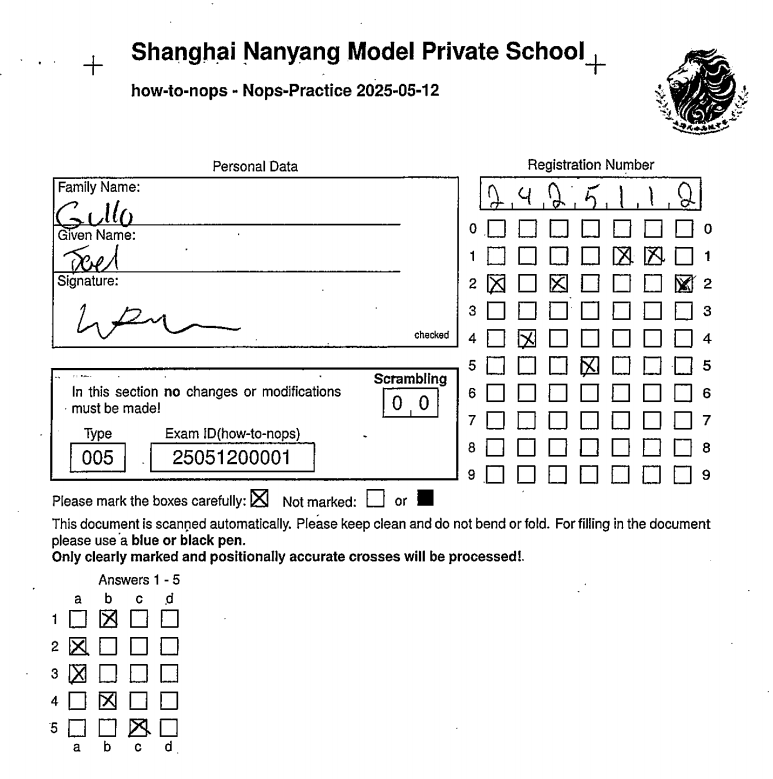
\includegraphics[width=0.5\linewidth]{phys11-exam-prep-nops-answer-sheet.png}
\end{figure}
\end{frame}

\begin{frame}{Answer Marking Standards}
\frametitle{Proper Marking Technique}
\begin{block}{Multiple Choice Answers}
\begin{itemize}
\item Mark exactly \textbf{one} answer per question
\item Use a clear X that fits completely inside the designated box
\item Ensure marks are dark and legible
\item Do not extend marks outside box boundaries
\end{itemize}
\end{block}

\begin{block}{Written Responses}
\begin{itemize}
\item Use designated answer boxes on separate page
\item Keep all work within box boundaries
\item Write legibly in blue or black pen
\item Include complete solutions and explanations
\end{itemize}
\end{block}
\end{frame}

\begin{frame}{Error Correction Protocol}
\frametitle{Managing Mistakes}
\begin{block}{Important: No Erasures Allowed}
Since pen marks cannot be erased, any marking errors require immediate attention.
\end{block}

\textbf{Incorrect approaches:}
\begin{itemize}
\item Crossing out wrong answers
\item Scribbling over incorrect marks  
\item Using correction fluid or tape
\end{itemize}

\textbf{Correct procedure:}
\begin{itemize}
\item Raise your hand immediately
\item Request a new answer sheet from the exam supervisor
\item Transfer all correct answers to the new sheet
\end{itemize}
\end{frame}

\begin{frame}{Pre-Submission Checklist}
\frametitle{Quality Assurance Review}
\begin{columns}
\begin{column}{0.5\textwidth}
\textbf{Personal Information:}
\begin{itemize}
\item[$\square$] Name written clearly
\item[$\square$] Signature provided
\item[$\square$] Registration number complete
\item[$\square$] Bubbles marked correctly
\end{itemize}
\end{column}

\begin{column}{0.5\textwidth}
\textbf{Answer Quality:}
\begin{itemize}
\item[$\square$] One mark per question
\item[$\square$] All marks clear and dark
\item[$\square$] No stray marks present
\item[$\square$] Sheet undamaged
\end{itemize}
\end{column}
\end{columns}

\begin{block}{Final Step}
Review your completed answer sheet thoroughly before submission to ensure optimal scanning results.
\end{block}
\end{frame}

\end{document}